\section{2D線段樹}
    \subsection{前言}
    又稱為樹套樹,有點像是二維前綴和,或是BIT。不過因為難很多
    所以放在進階資料結構篇。

    \subsection{概念}
    我們將$n$個線段樹,放進線段樹裡面。修改的時候先找到那一棵你要改的樹
    ,再修改裡面你要的節點。至於查詢,我們可以使用與1D相同的概念,查詢$O(\log n)$
    棵樹裡面的$O(\log m)$個節點。

    因此,兩種操作的時間複雜度都是$O(\log n \times \log m)$,通常來說$n \doteqdot m$,
    所以也可以記為$O(\log^{2}{(n)})$。

    \begin{figure}[ht]
        \centering
        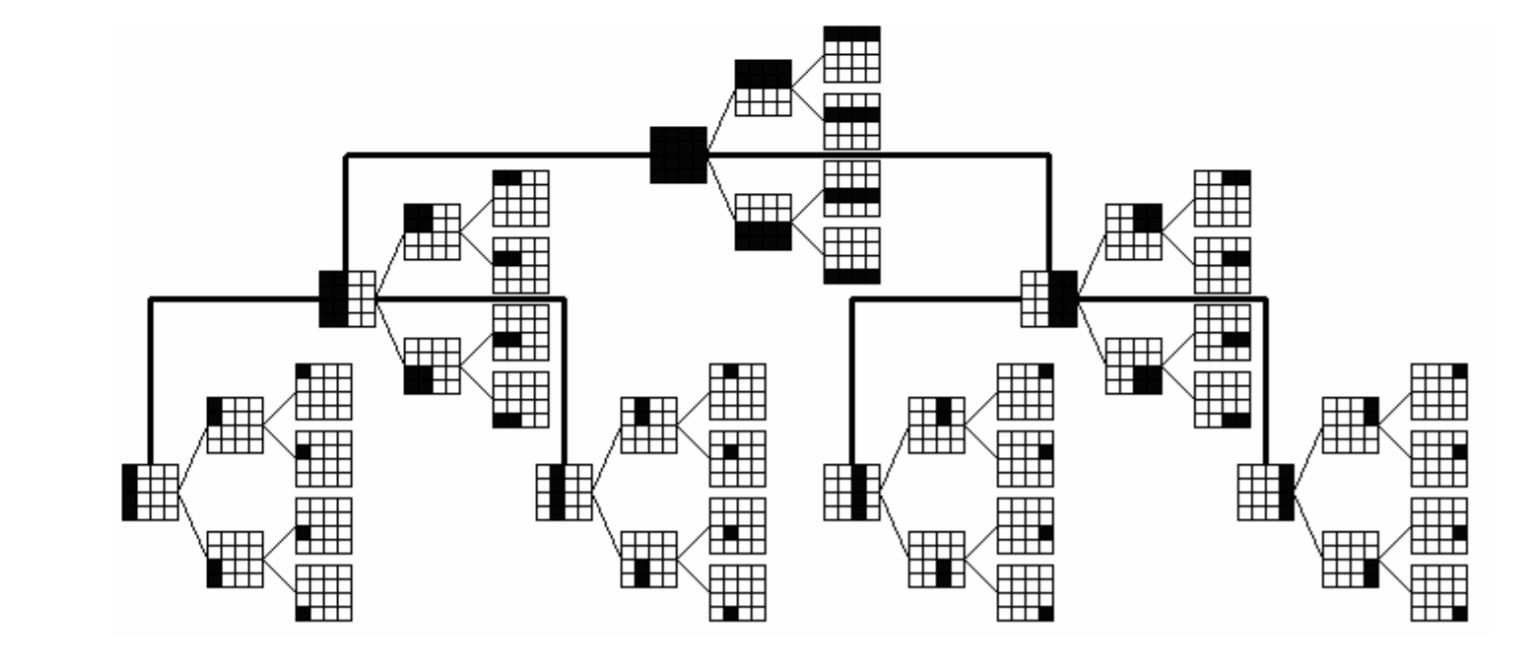
\includegraphics[width=\textwidth]{../Images/2DSeg1.png}
    \end{figure}

    \subsection{實作}
    我們會先實作seg1D,再用seg2D存放。

\begin{lstlisting}[caption=2D線段樹]
int N,M;
void amax(int &a,int b){
    a=max(a,b);
    return;
}

struct seg1D{
    int val=0;
    seg1D *lch=nullptr,*rch=nullptr;
    
    void pull(){
        val=0;
        if(lch) amax(val,lch->val);
        if(rch) amax(val,rch->val);
    }
    
    void modify(int x,int p,int lb=0,int rb=N){
        if(lb==rb){
            amax(val,p);
            return;
        }
        int mid=lb+rb>>1;
        
        if(x<=mid){
            if(!lch)lch=newseg1D;
            lch->modify(x,p,lb,mid);
        }

        if(mid<x){
            if(!rch) rch=new seg1D;
            rch->modify(x,p,mid+1,rb);
        }
        pull();
    }
    
    int query(int l,int r,int lb=0,int rb=N){
        if(l<=lb && rb<=r) return val;
        
        int mid=lb+rb>>1;
        int ret=0;
        if(l<=mid && lch) amax(ret,lch->query(l,r,lb,mid));
        if(mid<r && rch) amax(ret,rch->query(l,r,mid+1,rb));
        return ret;
    }
};

struct seg2D{
    seg1D seg;
    seg2D *lch=nullptr,*rch=nullptr;
    
    void modify(int x,int y,int p,int lb=0,int rb=N){
        seg.modify(y,p);
        if(lb==rb) return;
        
        int mid=lb+rb>>1;
        if(x<=mid){
            if(!lch) lch=new seg2D;
            lch->modify(x,y,p,lb,mid);
        }

        if(mid<x){
            if(!rch) rch=new seg2D;
            rch->modify(x,y,p,mid+1,rb);
        }
    }
    
    int query(int xl,int xr,int yl,int yr,int lb=0,int rb=N){
        if(xr<xl || yr<yl) return 0;
        if(xl<=lb && rb<=xr) return seg.query(yl,yr);
        int mid=lb+rb>>1;
        int ret=0;
        
        if(xl<=mid && lch) amax(ret,lch->query(xl,xr,yl,yr,lb,mid));
        if(mid<xr && rch) amax(ret,rch->query(xl,xr,yl,yr,mid+1,rb));
        return ret;
    }
};
\end{lstlisting}

    \subsection{誰說只能放線段樹}
    其實,你要把1D線段樹換成其他東西也可以,例如BIT,或是Treap(好期待)。

    \subsection{範例與練習}

    \problem ZJ c571 三維偏序

    給定 $n$ 個物件,每個物件有三個參數 $x_i, y_i, z_i$,
    請問最多可以選幾個物件,使得任意排序後,三個參數皆嚴格遞增。

    \problem CF19D Points

    \textbf{題目敘述}

    皮特和鮑勃發明了一個新奇的遊戲。鮑勃拿了一張紙,並在上面繪製了一個笛卡爾坐標系:點 $(0,0)$ 位於左下角,
    $x$ 軸向右延伸,$y$ 軸向上延伸。皮特給鮑勃提供了三種類型的請求:

    \begin{itemize}
        \item add x y:在紙上標記一個坐標為 $(x,y)$ 的點。對於每個此類型的請求,保證在請求時點 $(x,y)$ 尚未在紙上標記。
        \item remove x y:在紙上擦除先前標記的坐標為 $(x,y)$ 的點。對於每個此類型的請求,保證在請求時點 $(x,y)$ 已經在紙上標記。
        \item find x y:在紙上找到所有標記的點,這些點位於點 $(x,y)$ 的右上方。在這些點中,鮑勃選擇最左邊的點,如果不止一個,選擇最下面的點,並將其坐標返回給皮特。
    \end{itemize}
    
    鮑勃能夠回答10、100或1000個請求,但當請求的數量增加到 $2 \times 10^5$ 時,鮑勃無法處理。現在他需要一個能夠回答所有皮特請求的程式。請幫助鮑勃!

    \textbf{輸入說明}

    第一行輸入一個數字 $n$ ($1 \le n \le 2 \times 10^5$) ,表示請求的數量。接下來 $n$ 行描述了每個請求。add x y 表示標記一個點,
    remove x y 表示擦除一個點,find x y 表示查找底部最左邊的標記點。
    輸入中所有座標均為非負數且不超過 $10^9$。

    \textbf{輸出說明}

    對於每個 find x y 的請求,輸出一行結果,表示底部最左邊的標記點的座標。
    如果點 $(x,y)$ 的右上方沒有任何標記點,輸出 -1。

    \textbf{範例測試}

    \begin{tabular}{|m{7cm}|m{7cm}|}
        \hline
        範例輸入 1 & 範例輸出 1 \\
        \hline
        \verb|7| & \verb|1 1| \\
        \verb|add 1 1| & \verb|3 4| \\
        \verb|add 3 4| & \verb|1 1| \\
        \verb|find 0 0| & \\
        \verb|remove 1 1| & \\
        \verb|find 0 0| & \\
        \verb|add 1 1| & \\
        \verb|find 0 0| & \\
        \hline
    \end{tabular}

    \subsection{其他}

    二維線段樹幾乎不支援懶人標記,如果需要的話可以考如果需要的話可以考慮看看
    KD樹,或是四分樹。(有空我再研究看看)